\documentclass[a4paper,14pt]{extarticle}
\usepackage[utf8]{inputenc}
\usepackage[T2A]{fontenc}
\usepackage[russian]{babel}
\usepackage{amssymb}
\usepackage{fancyvrb}
\usepackage[fleqn]{amsmath}
\usepackage{amsthm}
\usepackage{amsmath}
\usepackage{hyperref} 
\usepackage{indentfirst}
\usepackage{caption}
\usepackage[left=3cm,right=1cm, top=2cm, bottom=2cm, bindingoffset=0cm]{geometry}
\hypersetup{
    colorlinks,
    citecolor=black,
    filecolor=black,
    linkcolor=black,
    urlcolor=black
}
% \textwidth = 16cm
% \usepackage{biblatex}
\usepackage{graphicx}
\usepackage{parskip}
% \addbibresource{bibliography.bib} 
\newtheorem{theorem}{Теорема}
\newenvironment{rowequmat}[1]{\left(\array{@{}#1@{}}}{\endarray\right)}

% \newenvironment{dwverbatim}{\begin{Verbatim}[fontsize=\scriptsize]} {\end{Verbatim}}

\sloppy
\parindent=0.5cm
\title{Курсовой проект}
\author{\copyright Андрей Румянцев}
\date{29 ноября 2016}
\selectlanguage{russian}
\allowhyphens
\begin{document}

\begin{titlepage}
    \linespread{1.1}
    \begin{center}
    \fontsize{15pt}{15pt}\selectfont
    МИНИСТЕРСТВО ОБРАЗОВАНИЯ РЕСПУБЛИКИ БЕЛАРУСЬ\\
    \vspace{0.5cm}
    БЕЛОРУССКИЙ ГОСУДАРСТВЕННЫЙ УНИВЕРСИТЕТ\\
    \vspace{0.5cm}
    ФАКУЛЬТЕТ ПРИКЛАДНОЙ МАТЕМАТИКИ И ИНФОРМАТИКИ\\
    \vspace{0.5cm}
    \fontsize{13pt}{13pt}\selectfont
    \textit{КАФЕДРА МАТЕМАТИЧЕСКОГО МОДЕЛИРОВАНИЯ И АНАЛИЗА ДАННЫХ}\\
    \vspace{3.0cm}
    \fontsize{18pt}{18pt}\selectfont

    \vspace{0.5cm}
    \textbf{Отчет}\\
    \textbf{о прохождении преддипломной практики}\\
    \vspace{0.5cm}
    \fontsize{16pt}{16pt}\selectfont
    ~~\\
    \end{center}
    \vspace{3.5cm}
    \fontsize{14pt}{14pt}\selectfont
    \hspace{-0.25cm}
    \def\arraystretch{1.2}
    \begin{tabular}{l@{\hspace{3.25cm}}l}
    ~~~~~~~~~~~~~~~~~~~~~~~~~~~~~~~~~~~~~~~~~~  & Румянцева Андрея Кирилловича\\
    ~~~~~~~~~~~~~~~~~~~~~~~~~~~~~~~~~~~~~~~~~~  & студента 4 курса, специальность\\
    ~~~~~~~~~~~~~~~~~~~~~~~~~~~~~~~~~~~~~~~~~~  & "прикладная математика"\\
    ~~~~~~~~~~~~~~~~~~~~~~~~~~~~~~~~~~~~~~~~~~  & \\
    ~~~~~~~~~~~~~~~~~~~~~~~~~~~~~~~~~~~~~~~~~~  & Руководитель практики:\\
    ~~~~~~~~~~~~~~~~~~~~~~~~~~~~~~~~~~~~~~~~~~  & зав. кафедрой ММАД, \\
    ~~~~~~~~~~~~~~~~~~~~~~~~~~~~~~~~~~~~~~~~~~  &  канд. физ.-мат. наук, доцент\\
    ~~~~~~~~~~~~~~~~~~~~~~~~~~~~~~~~~~~~~~~~~~  &Бодягин Игорь Александрович\\
    
    
    \end{tabular}
    \vspace{4.5cm}
    \begin{center}
    \fontsize{16pt}{16pt}\selectfont
    Минск, 2019
    \end{center}
\end{titlepage}

\newpage 
~~~~~~~~~
\thispagestyle{empty}
\addtocounter{page}{-1}
\mbox{}
\newpage


\tableofcontents
\newpage 

% \section*{Задание на практику}
\phantomsection
\addcontentsline{toc}{section}{Задание на практику}
\begin{itemize}
    \item Провести аналитический обзор литературы методов статистического анализа данных при наличии классифицированных наблюдений с искажениями.
    \item Реализовать альтернативные встречаемые в литературе методы статистического анализа данных при наличии классифицированных наблюдений с искажениями.
    \item Провести сравнительный анализ реализованного в ходе курсового проекта метода с альтернативными.
    \item Обобщить все реализованные методы с линейной на полиномиальную регрессию.
    \item Подготовить отчет по преддипломной практике.
\end{itemize}
% \newpage


\begin{center}
    \section*{ВВЕДЕНИЕ}
\end{center}
\phantomsection
\addcontentsline{toc}{section}{ВВЕДЕНИЕ}

В математической статистике широко используется регрессионная модель.
Существует несколько подходов для оценки параметров регрессии, но далеко не все устойчивы к возникновениям аномальных наблюдений, 
то есть таких наблюдений, которые не подчиняются общей модели. 
В реальной жизни аномальные наблюдения возникают постоянно. 
Такие наблюдения могут возникать по разным причинам: из-за ошибки измерения, из-за необычной природы входных данных.
По этой причине большинство методов просто неприменимо.
В прошлом веке в работах Хьюбера была заложена теория робастного оценивания.

Такие случаи, когда зависимые переменные наблюдаются с выбросами или с пропусками, хорошо исследованы \cite{OLSforGrouping}. Более сложный случай, когда вместо содержащих выбросы значений зависимой переменной наблюдаются номера классов(интервалов), в которые попадают эти наблюдения \cite{technometrics}.
Темой курсового проекта было \textit{"Статистическое оценивание параметров линейной регрессии с выбросами при наличии группирования наблюдений"}.

Целью преддипломной практики было продолжение исследования и улучшение оценок, построенных в 
курсовом проекте. 
 
\newpage

\section{Модель линейной регрессии с выбросами при наличии группирования наблюдений}
Рассмотрим модель линейной регрессии:
\begin{eqnarray}
    &\label{eq2}y_i= 
    \begin{pmatrix}
        \beta_0\\
        \beta_1\\
        \dots\\
        \beta_n
    \end{pmatrix}\times
    \begin{pmatrix}
        1\\
        x_{i1}\\
        \dots\\
        x_{in}
    \end{pmatrix}^{T}+ \varepsilon_i,\\
    &\label{eq6}y_i= f(x_i,\beta)+\varepsilon_i,\\
    &f(x_i,\beta)=\beta_0+\beta_1 x_{i1}+\beta_2 x_{i2}+\dots+\beta_n x_{in}.
\end{eqnarray}
Здесь $y_i$ -- зависимая переменная, $x_i=(x_{i1},x_{i2},\dots,x_{in})$ -- вектор регрессоров, \{$\beta_k, k=\overline{0,n}$\}-- коэффициенты линейной регрессии, а $\varepsilon_i$ -- случайная ошибка $i$-го эксперимента, распределение которой подчиняется нормальному закону с нулевым математическим ожиданием и дисперсией $\sigma^2$, $N$-объем выборки.
Согласно (\ref{eq6}) каждый $y_i$ принадлежит нормальному распределению:
\begin{eqnarray}
    \label{eq12} y_i=f(x_i,\beta)+\varepsilon_i \sim \mathcal{N}(f(x_i,\beta),\sigma^2).
\end{eqnarray}

Предполагается, что выборка содержит выбросы, описываемые следующим соотношением.
\begin{eqnarray}
    \label{eq3}y_i^{\widetilde{\varepsilon}}=(\xi_i)y_i+ (1-\xi_i)\eta_i,
\end{eqnarray}
где $\xi_i$ принимает значение, равное 1, с вероятностью $1-\widetilde{\varepsilon}$ и значение, равное 0, с вероятностью $\widetilde{\varepsilon}$:
\begin{eqnarray}\label{eq4}
    \begin{cases}
        P\{\xi_i=0\}=\widetilde{\varepsilon},\\
        P\{\xi_i=1\}=1-\widetilde{\varepsilon},
    \end{cases},
\end{eqnarray}
$\eta_i$-случайная величина из некоторого вообще говоря неизвестного распределения.

Параметр $\xi_i$ имеет следующий содержательный смысл: если $\xi_i=0$, то вместо истинного значения мы наблюдаем выброс, если $\xi_i=1$, то наблюдается истинное значение.
Переменную $\widetilde{\varepsilon}$ будем называть долей аномальных наблюдений. Величины $\xi_i, x_i$ и $\eta_i$ являются независимыми.

Пусть множество значений функции регрессии, т.е множество $\mathbb{R}$, разбито на $k$ непересекающихся полуинтервалов:
\begin{eqnarray}
    \mathbb{R}=(-\infty,a_1]\bigcup(a_1,a_2]\bigcup \dots \bigcup(a_{k-1},+\infty ).
\end{eqnarray}
Полученные полуинтервалы будем обозначать: $\nu_0,\dots,\nu_{k-1}$.

Предполагается, что каждый раз вместо истинного значения зависимой переменной $y_i$ наблюдается только номер интервала, в который это наблюдение попало.
Тогда для каждого $y_i$ будем наблюдать лишь номер полуинтервала $\mu_i$, в который он попал.
\begin{eqnarray}
    \label{eq13}\mu_i=j, \textup{если $y_i$} \in \nu_j.
\end{eqnarray}

В таком случае принято говорить, что имеет место группирование наблюдений, а сами наблюдения называются группироваными \cite{OLSforGrouping}.

В работе рассматривается задача оценивания параметров линейной регрессии с аномальными наблюдениями при наличии группирования наблюдений.

\section{Существующие способы оценивания параметров линейной регрессии с выбросами}
Для модели регрессии (\ref{eq2}), то есть для классической модели линейной регрессии, существует несколько способов оценивания параметров. Далее приведены некоторые из них.

\subsection{Метод наименьших квадратов}
Метод наименьших квадратов строится из предположения, что ошибки подчиняются нормальному закону распределения вероятностей:
\begin{eqnarray}
    \label{eq5}L\{\varepsilon_i\}=N_1(0,\sigma^2), i = \overline{1,n}.
\end{eqnarray}
Строится логарифмическую функцию правдоподобия. В силу (\ref{eq6}) имеем:
\begin{eqnarray}
    L\{y_i\}=N_1(f(x_i;\beta), \sigma^2).
\end{eqnarray}
Логарифмическая функция правдоподобия выглядит так\cite{Kharin}:
\begin{eqnarray}
    l(\beta)=\ln \prod_{i=1}^{n}(\frac{1}{\sqrt{2\pi}\sigma}e^{-\frac{(y_i-f(x_i;\beta))^2}{2\sigma^2}})&=&-\frac{1}{2}n\ln{2\pi\sigma^2}-\frac{1}{2\sigma^2}R^2(\beta),\\
    \label{eq7}R^2(\beta)=\sum_{i=1}^{n}(\delta y_i)^2&=&\sum_{i=1}^{n}(y_i-f(x_i,\beta))^2\geq 0.
\end{eqnarray}
Оценка методом наименьших квадратов называется такая оценка, которая миниимизирует  выражение (\ref{eq7}) такова:
\begin{eqnarray}
    \hat{\beta}=arg \min_{\beta}R^2(\beta).
\end{eqnarray}

Метод наименьших квадратов не считается робастным способом оценивания параметров линейной регрессии. Был проведен компьютерный эксперимент (раздел \ref{ss_1}), где оказалось, что вариации оценок не уменьшаются в случае увеличении объема выборки с аномальными наблюдениями.

\subsection{М-оценки}
М-оценки являются робастным способом оценивания параметров линейной регрессии с аномальными наблюдениями.
Швейцарский статистик П.Хьюбер предложил использовать М-оценки \cite{Kharin}, которые являются решениями экстремальных задач вида:
\begin{eqnarray}
    \sum_{i=1}^{n}\phi(x_t;\beta)\rightarrow \min_{\beta},
\end{eqnarray}
где $\phi(\cdot;\beta)$-некоторая функция, определяющая конкретный тип оценок и их точность.

Очевидно, что $\phi(\cdot;\beta)\equiv - \ln{p(\cdot;\beta)}$ дает обычную оценку максимального правдоподобия, построенную по модели без выбросов (\ref{eq2}).

Рассмотрим теперь некоторые способы выбора функции $\phi(\cdot;\beta)$ для решения экстремальной задачи в M-оценках.

Для начала определим:
\begin{eqnarray}
    u_i=y_i^{\widetilde{\varepsilon}}-(\beta_0+\beta_1 x_{i1}+\beta_2 x_{i2}+\dots+\beta_n x_{in}).
\end{eqnarray}
Тогда существует такие методы\cite{RobustRegression}:\hfill\break
\begin{center}
\begin{tabular}{ |p{3cm}|p{10cm} | }
    \hline
    \multicolumn{2}{|c|}{Способы выбора $\phi(\cdot;\beta)$} \\
    \hline
    Метод& Целевая функция\\
    \hline
    Метод Наименьших Квадратов&$\phi(\cdot;\beta)_{OLS}=u^2$\\
    \hline
    Хьюбера&$\phi(\cdot;\beta)_{H}=
        \begin{cases}
            \frac{1}{2}u^2, |u|\leq k,\\
            k|u|-\frac{1}{2}k^2, |u|>k
        \end{cases}$\\
    \hline
    Биквадратный& $\phi(\cdot;\beta)_{B}=
    \begin{cases}
        \frac{k^2}{6}(1-[1-(\frac{u}{k})^2]^3), |u|\leq k\\
        \frac{k^2}{6}, |u|>k
    \end{cases}$\\
    \hline
\end{tabular}
\end{center}

В разделе \ref{ss_1} приведено сравнение М-оценок с целевой функцией Хьюбера с оценками по Методу наименьших квадратов.

\newpage

\newpage
\section{Статистическое оценивание параметров линейной регрессии с выбросами при наличии группирования наблюдений}
Введем обозначение для функции распределения стандартного нормального закона:
\begin{eqnarray}
    \Phi(x)=\frac{1}{\sqrt{2}\sigma}\int_{-\infty}^{x}e^{\frac{-t^2}{2}}dt.
\end{eqnarray}

Тогда функцию распределения нормального закона с параметрами $\mu,\sigma^2$ можно представить как:
\begin{eqnarray}
    \label{eq10}F(x)=\Phi(\frac{x-\mu}{\sigma}),
\end{eqnarray}
где $\sigma = \sqrt{\sigma^2}$. \hfill\break
Обозначим:
\begin{eqnarray}
    \textup{erf}(x)=\frac{2}{\sqrt{\pi}}\int_0^{x}e^{-t^2}dt.
\end{eqnarray}
Тогда:
\begin{eqnarray}
    \Phi(x)= \frac{1}{2} \Big[1+\textup{erf}\Big(\frac{x}{\sqrt{2}} \Big) \Big].
\end{eqnarray}
Подставив полученные выражения в (\ref{eq10}) получим:
\begin{eqnarray}
    F(x)= \frac{1}{2} \Big[1+\textup{erf}\Big(\frac{x-\mu}{\sqrt{2}\sigma} \Big) \Big].
\end{eqnarray}
При модельных предположениях (\ref{eq12}) вероятность попадания $y_i$ в полуинтервал $\nu_j$ равна:
\begin{multline}
    P\{y_i\in\nu_j\}= F_{y_i}(a_{j+1})-F_{y_i}(a_{j})=\\
    =\begin{cases}
        \frac{1}{2}(\textup{erf}(\frac{a_{j+1}-f(x_i,\beta)}{\sqrt{2}\sigma})-\textup{erf}(\frac{a_{j}-f(x_i,\beta)}{\sqrt{2}\sigma})),~j=\overline{1,k-2}\\
        \frac{1}{2}(1+\textup{erf}(\frac{a_{1}-f(x_i,\beta)}{\sqrt{2}\sigma})),~j=0\\
        -\frac{1}{2}(1+\textup{erf}(\frac{a_{k-1}-f(x_i,\beta)}{\sqrt{2}\sigma})),~j=k-1
    \end{cases}.
\end{multline}
Понятно, что:
\begin{eqnarray}
    P(\mu_i=j)=P(y_i\in \nu_{\mu_i}).
\end{eqnarray}

Решается задача статистического оценивания параметров модели (\ref{eq2}) \{$\beta_k, k=\overline{0,n}$\} по известным группированным наблюдениям. Здесь наличие аномальных наблюдений не учитывается.

Для этого построим функцию правдоподобия:
\begin{eqnarray}
    \label{eq22}\label{eq23}&l(\beta,\sigma^2, \mu_1,\dots, \mu_{N})=\sum\limits_{i=1}^{N}\ln(P(y_i\in \nu_{\mu_i}))=\\
    &=\sum\limits_{i=1}^{N}\ln\begin{cases}
        \frac{1}{2}(\textup{erf}(\frac{a_{j+1}-f(x_i,\beta)}{\sqrt{2}\sigma})-\textup{erf}(\frac{a_{j}-f(x_i,\beta)}{\sqrt{2}\sigma})),~i=\overline{1,k-2}\\
        \frac{1}{2}(1+\textup{erf}(\frac{a_{1}-f(x_i,\beta)}{\sqrt{2}\sigma})),~i=0\\
        -\frac{1}{2}(1+\textup{erf}(\frac{a_{k-1}-f(x_i,\beta)}{\sqrt{2}\sigma})),~i=k-1
    \end{cases},
\end{eqnarray}
где:
\begin{eqnarray}
    \textup{erf}(x)=\frac{2}{\sqrt{\pi}}\int_0^{x}e^{-t^2}dt.
\end{eqnarray}

Для максимизации функции правдоподобия решим систему уравнений:
\begin{eqnarray}
    \label{eq24}\frac{\delta l}{\delta \beta}=0_{n+1},
\end{eqnarray}
где:
\begin{multline}
    \label{eq27}\frac{\delta l}{\delta \beta}=\frac{\delta \sum\limits_{i=1}^{N}\ln P(y_i\in \nu_{\mu_i})}{\delta \beta}=~\\
    =\frac{\delta \sum\limits_{i=1}^{N} \ln(\frac{1}{2}(\textup{erf}(\frac{a_{\mu_i+1}-f(x_i,\beta)}{\sqrt{2}\sigma})-\textup{erf}(\frac{a_{\mu_i}-f(x_i,\beta)}{\sqrt{2}\sigma})) )         }{\delta \beta}=~\\
    =  \sum\limits_{i=1}^{N}\Big((1-(\delta_{\mu_i 0}+\delta_{\mu_i k-1}))\frac{(\textup{erf'}(\frac{a_{\mu_i+1}-f(x_i,\beta)}{\sqrt{2}\sigma})-\textup{erf'}(\frac{a_{\mu_i}-f(x_i,\beta)}{\sqrt{2}\sigma}))}{ (\textup{erf}(\frac{a_{\mu_i+1}-f(x_i,\beta)}{\sqrt{2}\sigma})-\textup{erf}(\frac{a_{\mu_i}-f(x_i,\beta)}{\sqrt{2}\sigma}))}+~\\
    +(\delta_{\mu_i 0}+\delta_{\mu_i k-1})\frac{\textup{erf'}(\frac{a_{\mu_i}-f(x_i,\beta)}{\sqrt{2}\sigma})}{(1+\textup{erf}(\frac{a_{\mu_i}-f(x_i,\beta)}{\sqrt{2}\sigma}))}\Big)  (-1) \frac{\delta f(x_i,\beta)}{\delta \beta} )=~
\end{multline}
\begin{multline}
    \nonumber 
    =-\sum_{i=1}^{N}\begin{pmatrix}
        1\\
        x_{i1}\\
        \dots\\
        x_{in}
    \end{pmatrix}\times  \Big((1-(\delta_{\mu_i 0}+\delta_{\mu_i k-1}))\frac{(\textup{erf'}(\frac{a_{\mu_i+1}-f(x_i,\beta)}{\sqrt{2}\sigma})-\textup{erf'}(\frac{a_{\mu_i}-f(x_i,\beta)}{\sqrt{2}\sigma}))}{ (\textup{erf}(\frac{a_{\mu_i+1}-f(x_i,\beta)}{\sqrt{2}\sigma})-\textup{erf}(\frac{a_{\mu_i}-f(x_i,\beta)}{\sqrt{2}\sigma}))}+~\\
    +(\delta_{\mu_i 0}+\delta_{\mu_i k-1})\frac{\textup{erf'}(\frac{a_{\mu_i}-f(x_i,\beta)}{\sqrt{2}\sigma})}{(1+\textup{erf}(\frac{a_{\mu_i}-f(x_i,\beta)}{\sqrt{2}\sigma}))}\Big) .
\end{multline}
$\delta_{ij} = \{1, i=j; 0, i\neq j\}$ - символ Кронекера, $0_{n+1}=(0, \dots, 0)^T$ - вектор размерности $n+1$ состоящий из одних нулей.

В полученном уравнении используется функция $\textup{erf}(x)$ и ее производная. Для вычисления значений этой фунции существует таблица значений и приближение аналитической функцией \cite{Winitzki}.
Будем использовать приближение для функции $\textup{erf}(x)$:
\begin{eqnarray}
    \label{eq25}(\textup{erf} (x))^2&\approx& 1- \exp(-x^2 \frac{\frac{4}{\pi}+ax^2}{1+ax^2}),\\
    \nonumber a&=&\frac{8}{3\pi}\frac{3-\pi}{\pi -4}.
\end{eqnarray}
Оно считается достаточно точным для $x$ близких к $0$ и к $\infty$ \cite{Winitzki}. \hfill\break

Найдем производную для этого приближения:
\begin{eqnarray}
    \label{eq26}\textup{erf}'(x) = \exp(-x^2 \frac{\frac{4}{\pi}+ax^2}{1+ax^2}) \frac{-2x\frac{\frac{4}{\pi}+ax^2}{1+ax^2}+(2ax^3)\frac{\frac{4}{\pi}+ax^2}{1+ax^2}-\frac{2ax^3}{1+ax^2}}{2\sqrt{1- \exp(-x^2 \frac{\frac{4}{\pi}+ax^2}{1+ax^2})}}.
\end{eqnarray}

Подставив  выражения (\ref{eq25})-(\ref{eq26}) в (\ref{eq24}), получим уравнение, которое будем решать методом секущих.


\subsection{Метод секущих}\label{sec4_2}
Так как мы не можем привести систему $ \frac{\delta l}{\delta \beta}=0$ к виду, удобному для итерации, то нам придется искать ее нули с помощью метода секущих \cite{NumericalMethods}.
Введем вектор ошибки $\check{\varepsilon}^{(k)}=\beta^{*}-\beta^{(k)}$. Тогда для его определения имеем:
\begin{eqnarray}
    \frac{\delta l (\beta^{(k)}+\check{\varepsilon}^{(k)})}{\delta \beta}=0.
\end{eqnarray}
Строя разложение левой части по формуле Тейлора и ограничиваясь лишь линейными членами\cite{NumericalMethods}, будем иметь систему:
\begin{eqnarray}
    \frac{\delta }{\delta \beta}\frac{\delta l (\beta^{(k)}}{\delta \beta}\Delta \beta^{(k)}=-\frac{\delta l (\beta^{(k)})}{\delta \beta}.
\end{eqnarray}
Вторая производная функции $l$ приближается с помощью выражения:
\begin{eqnarray}
    \frac{\delta }{\delta \beta_j}\frac{\delta l(\beta_1^{(k)},\dots, \beta_n^{(k)}) }{\delta \beta}\approx \frac{\frac{\delta l(\beta_1^{(k)},\dots,\beta_j^{(k)},\dots, \beta_n^{(k)}) (\beta^{(k)}}{\delta \beta}-\frac{\delta l(\beta_1^{(k)},\dots,\beta_j^{(k-1)},\dots, \beta_n^{(k)}) (\beta^{(k)}}{\delta \beta}}{\beta_j^{(k)}-\beta_j^{(k-1)}}.
\end{eqnarray}
Если матрица $\frac{\delta }{\delta \beta}\frac{\delta l (\beta^{(k)}}{\delta \beta}$ невырожденная (а в нашем случае она диагональная), то из этой системы можно единственным образом найти $\Delta \beta^{(k)}$ и построить приближение:
\begin{eqnarray}
    \beta^{(k+1)}=\beta^{(k)}+\Delta \beta^{(k)}.
\end{eqnarray}

Согласно \cite{NumericalMethods} метод секущих в общем случае обладает квадратичной сходимостью.

Одним из минусов метода секущих является то, что он требует два начальных приближения, т.е. отрезок, где, как мы предполагаем, находится точное значение параметров регрессии.
Условием остановки метода секущих будем задавать такое, что разница значений логарифмической функции правдоподобия $l$ на двух соседних итерациях не более некоторой заданной величины.
Теперь имеем нули производной функции $l$, а также ее значения на границе отрезка $[a,b]$.
Переберем эти значения и таким образом найдем значение вектора $\hat{\beta}$, где она достигает своего максимального значения.

\subsection{Переклассификация выборки}

Для уменьшения влияния выбросов будем использовать переклассификацию выборки.
Идея заключается в том, что аномальные наблюдения с большей вероятностью попадают не в те интервалы, в которые попадают истинные наблюдения. 
При этом переклассификация может помочь отнести аномальные наблюдения к истинным классам и улучшить качество оценивания.


В ходе выполнения дипломной работы было испробовано несколько способов переклассификации выборки. Один из них: метод $K$-ближайших соседей. 

\subsubsection{Метод $K$-ближайших соседей}
На первом этапе для каждого вектора $x_i$ задан класс $\mu_i$: т.е. пара $(x_i,\mu_i)$.
Далее выполним переклассификацию выборки. 
Для этого построим новую выборку такого же объема $N$.
Пройдемся по каждому элементу $(x_i, \mu_i)$ выборки и для этого наблюдения построим новое:
\begin{eqnarray}
    (x_i, \check{\mu}_i),
\end{eqnarray}
где $\check{\mu}_i$ получен по методу $K$-ближайших соседей\cite{NEAREST_NEIGHBOR}.\hfill\break
\begin{eqnarray}
    \check{\mu}_i = \arg\max_j \sum_{k \in V_i,~k\neq i} \delta_{\check{\mu}_k j}~,
\end{eqnarray}
где $V_i$ множество индексов $l$ первых $K$ векторов $x_l$, отсортированных по возрастанию расстояния до вектора $x_i$.

После переклассификации выборки, к ней применяется функция правдоподобия (\ref{eq22}), только теперь с использованием новых классов $\check{\mu}_i$ вместо $\mu_i$. 
Она аналогично максимизируется и в итоге находится новая оценка параметров $\hat{\beta}$.

В ходе экспериментов (раздел \ref{sec_exp}) оказалось, что метод $K$ ближайших соседей исправляет очень мало ошибочных классов в выборке, поэтому было решено использовать другой метод переклассификации.

\subsubsection{Переклассификация с использованием Локального уровня выброса и Случайного леса}
Идея метода заключается в следующем: определим в выборке такие наблюдения, которые, вероятно, являются аномальными с помощью какого-либо способа. После этого выберем наблюдения, которые не определились как аномальные.
Обучим на полученных наблюдениях классификатор. После этого с помощью обученного классификатора переклассифицируем те наблюдения, которые определились как аномальные. В итоге получим выборку, которую будем использовать при решении уравнения (\ref{eq22}) \cite{LOF}.

Для определения аномальных наблюдений можно использовать Локальный уровень выброса. Метод был предложен Маркусом М.~Бройнигом, Гансом-Петер~Кейгелем, Реймондом~Т.~НГ и Ёргом Сандером в 2000 году. Аномальные наблюдения находятся с помощью измерения локального отклонения точек с учётом их соседей.
Метод основан на концепте локальной плотности достижимости, где локальная плотность достижимости вычисляется с учётом ближайших $K$ соседей, расстояние до которых используется для вычисления плотности. Сравнивая локальную плотность точки с локальной плотностью соседей можно определять точки, которые обладают значительно меньшей локальной плотностью по сравнению с соседями. Такие точки будем считать выбросами.

Пусть $x_i$ является некоторой точкой выборки. Определим $\rho(x_i, x_l)$ -- расстояние от точки $x_i$ до точки $x_l$ (будем использовать Евклидову метрику), $\rho_k(x_i)$ -- расстояние от точки $x_i$ до её $K$-го соседа. 
Аналогично методу $K$-ближайших соседей обозначим множество индексов $k$ первых $K$ векторов $x_k$, отсортированных по возрастанию расстояния до вектора $x_i$ через $V_i$.
Использользуя введеные величины зададим:
\begin{eqnarray}
    \hat{\rho}_k(x_i, x_l) = \max\{\rho_k(x_l), \rho(x_i, x_l)\}.
\end{eqnarray}

Такую величину можно интерпретировать как истинное расстояние от точки $x_l$ до точки $x_i$ если $x_l$ не входит в ее $K$ ближайших соседей или расстояние до точки $x_{V_{l_K}}$ в противном случае. 
Данная величина введена для того, чтобы более стабильно вычислять расстояние для тех значений, которые входят в $K$-ближайших соседей точки $x_l$. 

Заметим, что введенная величина не обладает свойством симметричности.

Локальную плотность достижимости зададим выражением:
\begin{eqnarray}
    \textup{lrd}_k(x_i) = 1 / \bigg(\frac{\sum\limits_{l\in V_i}\hat{\rho}_k(x_i, x_l)}{|V_i|}\bigg).
\end{eqnarray}

Теперь можно задать величину:
\begin{eqnarray}
    \textup{LOF}_k(x_i) = \frac{\sum\limits_{l\in V_i}\frac{\textup{lrd}_k(x_l)}{\textup{lrd}_k(x_i)}}{|V_i|}.
\end{eqnarray}
Она является средней локальной плотностью достижимости соседей точки $x_i$ по отношению к своей локальной плотности достижимости точки $x_i$. 

По полученному значению можно судить \cite{LOF}, является ли наблюдение $x_i$ выбросом или нет:
\begin{itemize}
    \item $\textup{LOF}_k(x_i)\sim 1$   -- означает, что у наблюдения $x_i$ такая же плотность как и у его соседей;\\
    \item $\textup{LOF}_k(x_i)<1$  -- означает, что у наблюдения $x_i$ большая плотность чем у его соседей (наблюдение - истинное);\\
    \item $\textup{LOF}_k(x_i)>1$ -- означает, что у наблюдения $x_i$ меньшая плотность чем у его соседей (наблюдение - выброс).
\end{itemize}

Таким образом найдем аномальные наблюдения в выборке.

Теперь обучим классификатор на предполагаемых истинных значениях выборки. Воспользуемся алгоритмом классификации на основе Случайного леса \cite{RANDOM_FORESTS}. Построим по выборке несколько деревьев решений. 
Применим обученный классификатор к каждому аномальному наблюдению. Тот класс, к которому отнесло наибольшее количество простроенных деревьев решений будем считать истинным классом данного аномального наблюдения.

В ходе компьютерных экспериментов была построена таблица подходящих значений $K$ для заданной длины интервала и объема выборки (раздел \ref{ss3_3_2} таблица \ref{tab2}).

\newpage
\subsection{Альтернативные оценки параметров модели}
Рассмотрим альтернативный метод оценивания параметров модели регрессии, основанный на замене группированных наблюдений серединами соответствующих интервалов. 
Такой метод встречается в литературе, например в \cite{interval_valued}.

Метод заключается в следующем:
пусть имеется $\mu_i$ - номер полуинтервала, в который попало очередное наблюдение $y_i$. Ему соответствует полуинтервал $\nu_{\mu_i}$ (из (\ref{eq13})), т.е. полуинтервал:
\begin{eqnarray}
    y_i\in (a_{\nu_{\mu_i}},a_{\nu_{\mu_i}+1}], i = \overline{1,N}
\end{eqnarray}
(считаем что $a_1<y_i<a_{k-1}, i=\overline{1,N}$, т.е $1\leq\mu_i\leq k-2$).

Найдем центральную точку этого интервала, т.е. точку
\begin{eqnarray}
    \check{y_i} = \frac{a_{\nu_{\mu_i}} + a_{\nu_{\mu_i}+1}}{2}.
\end{eqnarray}

Построим для всех значений функции регрессии $y_i$ значения $\check{y_i}$.
Будем использовать в качестве значений функции регрессии полученные значения $\check{y_i}$, а в качестве регрессоров $x_i$ и построим МНК оценки параметров $\beta$.

Теперь имеет три вида оценок: оценки максимального правдоподобия, оценки максимального правдоподобия с переклассификацией, МНК по серединам интервалов. 
\newpage
\subsection{Полиномиальная регрессия}
Введем теперь модель полиномиальной регрессии.

\begin{equation}
    \begin{array}{c}
        \label{eq28}y_i=\beta_0+\beta_1 x_{i1}^1+\beta_2 x_{i2}^2+\dots+\beta_n x_{in}^n+\varepsilon_i, i=\overline{1,N},\\
        y_i = \sum\limits_{l=1}^{n} x_{il}^{l-1} + \varepsilon_i, i=\overline{1,N},\\
        y_i= f(x_i,\beta)+\varepsilon_i,\\
        f(x_i,\beta)=\beta_0+\beta_1 x_{i1}^1+\beta_2 x_{i2}^2+\dots+\beta_n x_{in}^n.
    \end{array}
\end{equation}
В случае полиномиальной регрессии также справедливо:
\begin{eqnarray}
    y_i\sim \mathcal{N}(f(x_i,\beta),\sigma^2).
\end{eqnarray}

Поскольку оценки строились путём максимизирования функции:
\begin{eqnarray}
    &l(\beta,\sigma^2, \nu_0,\dots, \nu_{k-1})=\sum_{i=1}^{N}\ln(P(y_i\in \nu_{\mu_i}))=\\
    &=\sum\limits_{i=1}^{N}\ln\begin{cases}
        \frac{1}{2}(\textup{erf}(\frac{a_{j+1}-f(x_i,\beta)}{\sqrt{2}\sigma})-\textup{erf}(\frac{a_{j}-f(x_i,\beta)}{\sqrt{2}\sigma})),~i=\overline{1,k-2},\\
        \frac{1}{2}(1+\textup{erf}(\frac{a_{1}-f(x_i,\beta)}{\sqrt{2}\sigma})),~i=0,\\
        \frac{1}{2}(1+\textup{erf}(\frac{a_{k-1}-f(x_i,\beta)}{\sqrt{2}\sigma})),~i=k-1,
    \end{cases}
\end{eqnarray}
а функция правдоподобия максимизировалась путём решения системы уравнений:
\begin{eqnarray}
    \frac{\delta l}{\delta \beta}=0,
\end{eqnarray}
которая примет вид:
\begin{multline}
    \frac{\delta l}{\delta \beta}=\frac{\delta \sum\limits_{i=1}^{N}\ln P(y_i\in \nu_{\mu_i})}{\delta \beta}=~\\
    =\frac{\delta \sum\limits_{i=1}^{N} \ln(\frac{1}{2}(\textup{erf}(\frac{a_{\mu_i+1}-f(x_i,\beta)}{\sqrt{2}\sigma})-\textup{erf}(\frac{a_{\mu_i}-f(x_i,\beta)}{\sqrt{2}\sigma})) )         }{\delta \beta}=~\\
    =  \sum\limits_{i=1}^{N}\Big((1-(\delta_{\mu_i 0}+\delta_{\mu_i k-1}))\frac{(\textup{erf'}(\frac{a_{\mu_i+1}-f(x_i,\beta)}{\sqrt{2}\sigma})-\textup{erf'}(\frac{a_{\mu_i}-f(x_i,\beta)}{\sqrt{2}\sigma}))}{ (\textup{erf}(\frac{a_{\mu_i+1}-f(x_i,\beta)}{\sqrt{2}\sigma})-\textup{erf}(\frac{a_{\mu_i}-f(x_i,\beta)}{\sqrt{2}\sigma}))}+~\\
    +(\delta_{\mu_i 0}+\delta_{\mu_i k-1})\frac{\textup{erf'}(\frac{a_{\mu_i}-f(x_i,\beta)}{\sqrt{2}\sigma})}{(1+\textup{erf}(\frac{a_{\mu_i}-f(x_i,\beta)}{\sqrt{2}\sigma}))}\Big)  (-1) \frac{\delta f(x_i,\beta)}{\delta \beta} )=~
\end{multline}
\begin{multline}
    \nonumber 
    =-\sum_{i=1}^{N}\begin{pmatrix}
        1\\
        x_{i1}^1\\
        \dots\\
        x_{in}^n
    \end{pmatrix}\times  \Big((1-(\delta_{\mu_i 0}+\delta_{\mu_i k-1}))\frac{(\textup{erf'}(\frac{a_{\mu_i+1}-f(x_i,\beta)}{\sqrt{2}\sigma})-\textup{erf'}(\frac{a_{\mu_i}-f(x_i,\beta)}{\sqrt{2}\sigma}))}{ (\textup{erf}(\frac{a_{\mu_i+1}-f(x_i,\beta)}{\sqrt{2}\sigma})-\textup{erf}(\frac{a_{\mu_i}-f(x_i,\beta)}{\sqrt{2}\sigma}))}+~\\
    +(\delta_{\mu_i 0}+\delta_{\mu_i k-1})\frac{\textup{erf'}(\frac{a_{\mu_i}-f(x_i,\beta)}{\sqrt{2}\sigma})}{(1+\textup{erf}(\frac{a_{\mu_i}-f(x_i,\beta)}{\sqrt{2}\sigma}))}\Big),
\end{multline}
то построенные оценки также применимы и для полиномиальной регрессии.

Также как и в случае линейной регрессии считаем, что выборка содержит выбросы, т.е., аналогично:
\begin{eqnarray}
    y_i^{\widetilde{\varepsilon}}=(\xi_i)y_i+ (1-\xi_i)\eta_i,
\end{eqnarray}
здесь $y_i$ задаются формулой (\ref{eq28}).


\newpage

\section{Компьютерные эксперименты}\label{sec_exp}
\subsection{График рассеяния зависимой пеменной и регрессоров}
Чтобы зрительно представлять, как выбросы влияют на функцию регрессии, был построен график рассеяния зависимой переменной и регрессоров: $(y_i^{\widetilde{\varepsilon}}, x_i)$.

Бралась выборка объема $N = 1000$. Доля выбросов $\widetilde{\varepsilon}$ равнялась $0.08$. 
Параметры регрессии выбирались $(90, 4)^T$. 
Регрессоры $x_i$ выбирались из равномерного распределения $\sim U(-5,5)$. 
Ошибки экспериментов подчинялись нормальному закону распределения с параметрами $(0, 16)$. Выбросы подчинялись нормальному распрелению с параметрами $(100, 100)$. 

\begin{figure}[h!]
    \centering
    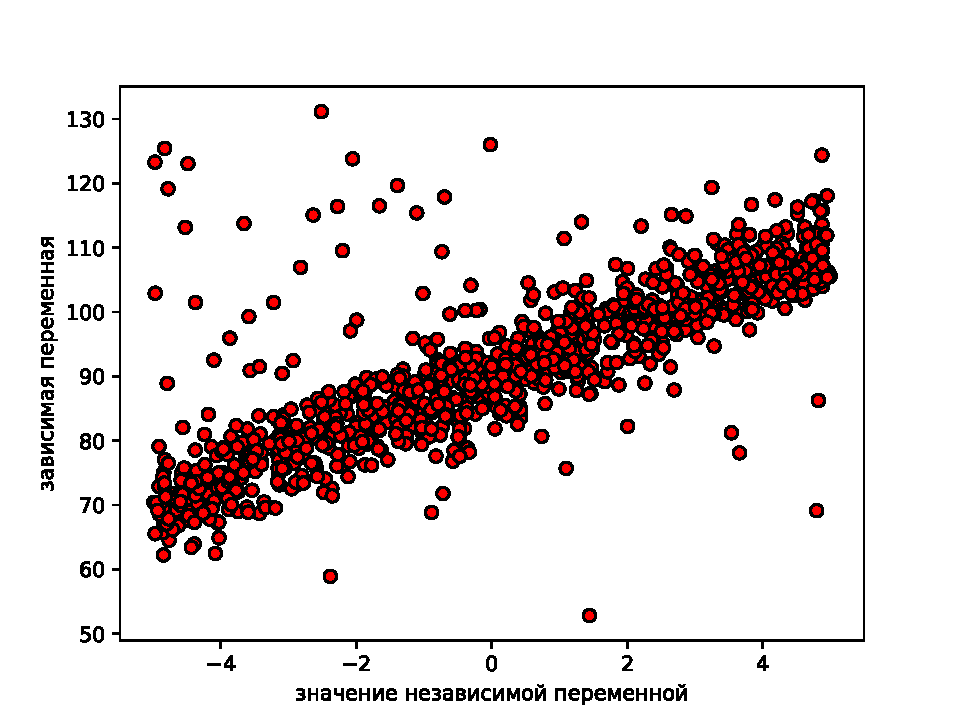
\includegraphics[width=100mm]{../images/scatter.pdf}
    \caption{График рассеяния $(y_i^{\widetilde{\varepsilon}}, x_i)$\label{overflow}}
    \label{pic_scatter}
\end{figure}

На рисунке \ref{pic_scatter} видно, что часть аномальных наблюдений сильно отстоит от генеральной совокупности наблюдений и поэтому вносят сильное искажение в результирующие группированые наблюдения, но при этом, по всей видимости, может быть выявлена при переклассификации.
Остальная часть аномальных наблюдений ''смешивается'' с генеральной совокупностью и поэтому плохо выявляется при переклассификации.

\newpage


\subsection{Вариации оценок МНК и М-оценок в случае линейной регрессии с выбросами}\label{ss_1}
Далее было проведено сравнение, как ведет себя классический метод и робастный метод в случае возникновения аномальных наблюдений в выборке.

На следующих двух графиках изображено изменение вариаций М-оценок и МНК оценок при увеличении объема выборки.

\begin{figure}[h!]
    \centering
    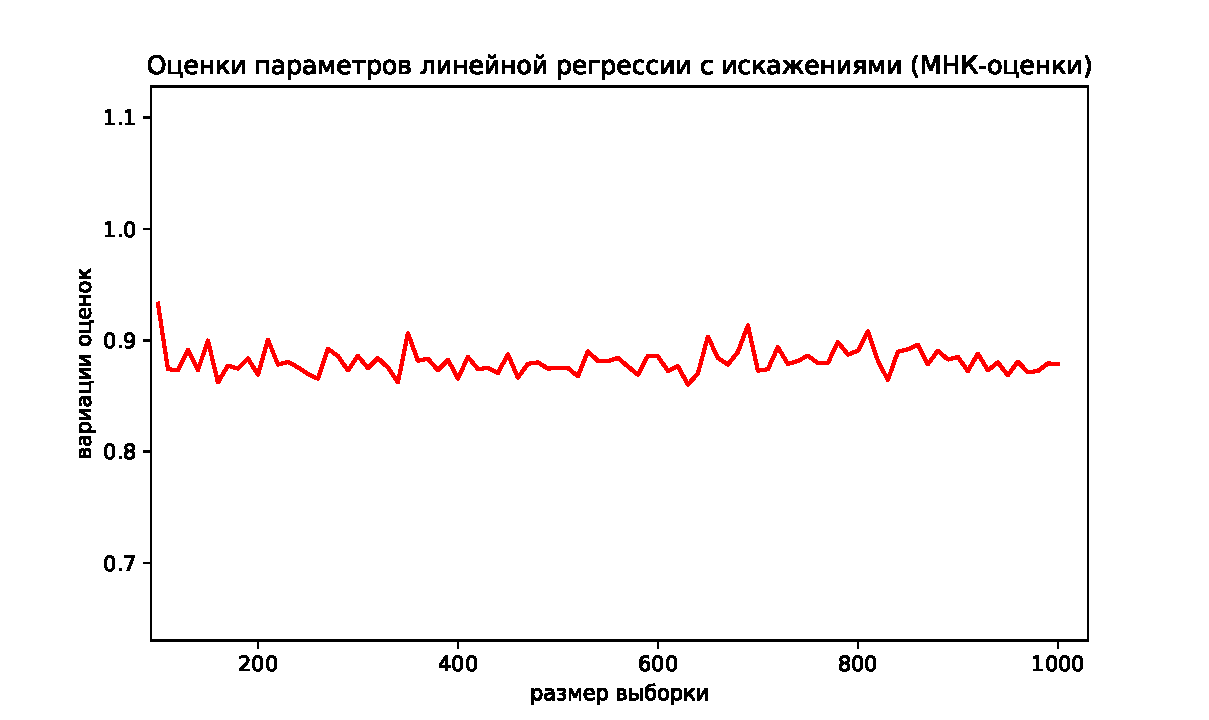
\includegraphics[width=100mm]{../images/OLS.pdf}
    \caption{Вариации оценок МНК в зависимости от объема выборки при постоянной доле выбросов\label{overflow}}
    \label{pic_ols}
\end{figure}

\begin{figure}[h!]
    \centering
    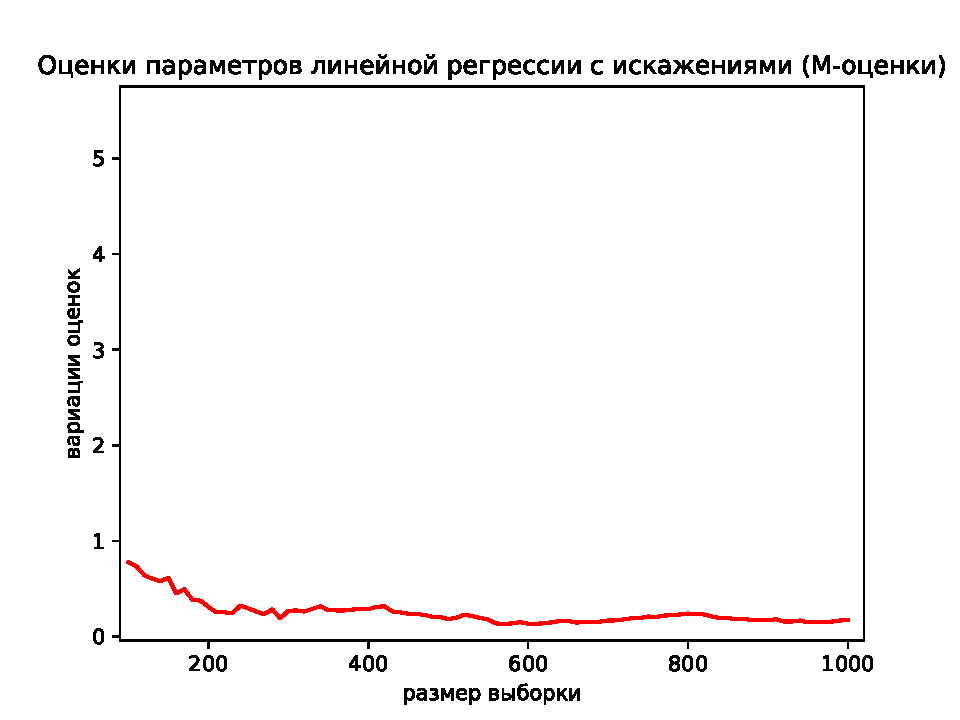
\includegraphics[width=100mm]{../images/RLM(1).pdf}
    \caption{Вариации оценок М-оценок в зависимости от объема выборки при постоянной доле выбросов\label{overflow}}
\end{figure}

Объем выборки изменялся от $N=100$ до $N=1000$. 
Доля выбросов $\widetilde{\varepsilon}$ равнялась $0.08$. 
Параметры регрессии выбирались $(90, 4)^T$. 
Регрессоры $x_i$ выбирались из равномерного распределения $\sim U(-5,5)$. 
Ошибки экспериментов подчинялись нормальному закону распределения с параметрами $(0, 16)$. Выбросы подчинялись нормальному распрелению с параметрами $(100, 100)$. 

На графиках видно, что робастные М-оценки в отличие от оценок МНК сходятся с увеличением объема выборки. 
Рисунок \ref{pic_ols} показывает, почему важна задача построения робастных методов оценивания параметров регрессии: классический метод (оценки МНК) не сходится при увеличении объема выборки.

\subsection{Вариации оценок без переклассификации}
Далее был проведен похожий эксперимент на эксперимент в пункте \ref{ss_1}, но кроме аномальных наблюдений присутствовало группирование выборки. Использовались построенные ОМП-оценки, но не применялась переклассификация выборки. 

Объем выборки $N$ изменялся от $N_1=140$ до $N_2=300$, при этом выборка дополнялась, а не генерировалась новая. Использовалась модель линейной регрессии. Доля выбросов была постоянна и равнялась $\widetilde{\varepsilon}=0.08$. 
Регрессоры $x_i$ были из равномерного распределения $U(-5,5)$.  Параметры регрессии были постоянными и равнялись $\beta=(90,4)^T$. Ошибки эспериментов $\varepsilon_i\sim \mathcal{N}(0,16)$.
На графики изображено изменение вариаций оценок при увеличении объема выборки.
\begin{figure}[hb]
    \centering
    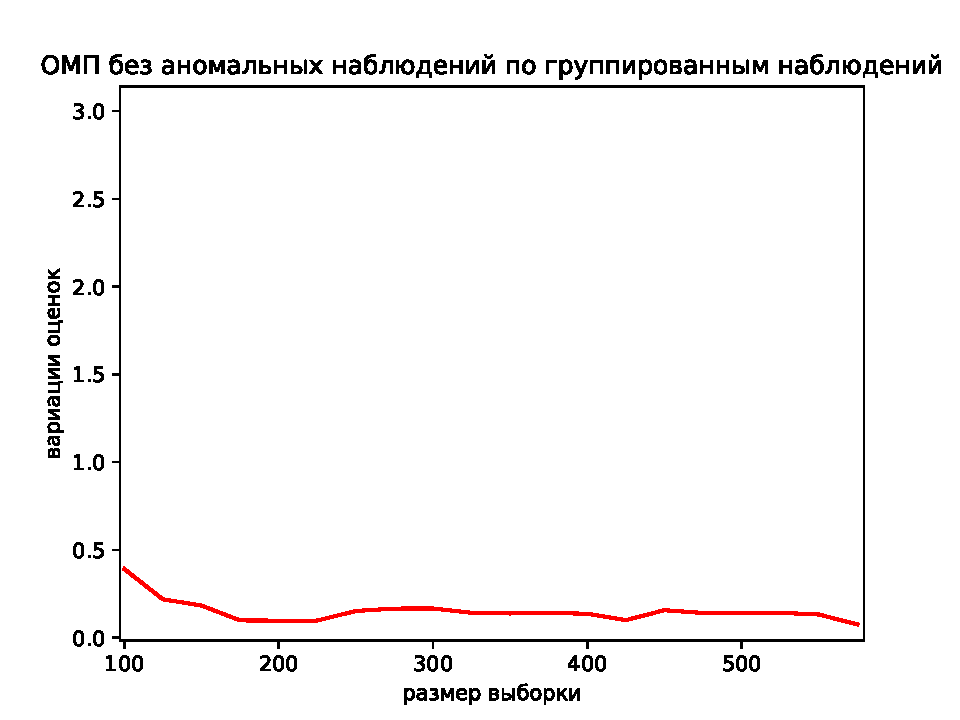
\includegraphics[width=100mm]{../images/MLE_no_outliers(2).pdf}
    \caption{Зависимость вариаций от размера выборки\label{overflow}}
    \label{pic6}
\end{figure}

С увеличением объема выборки построенные ОМП-оценки сходятся, но так как в выборке присутствуют аномальные наблюдения, скорость сходимости метода невелика и дисперсия вариаций оценок очень большая. 

\subsection{Графики рассеяния оценок в случае использования метода K-ближайших соседей для переклассификации}
Далее к выборке с аномальными наблюдениями с группированием применялась переклассификации, а после этого применялись построенные ОМП-оценки.

На следующих двух графиках (рис. \ref{pic4} - рис. \ref{pic5}) изображена диаграмма рассеяния, если для переклассификации выборки выбран метод $K$-ближайших соседей.

Для построения рисунка \ref{pic4} генерировались выборки объема $N = 1000$. Доля выбросов $\widetilde{\varepsilon}$ равнялась $0.08$. 
Параметры регрессии выбирались $(90, 4)^T$. 
Регрессоры $x_i$ выбирались из равномерного распределения $\sim U(-5,5)$. 
Ошибки экспериментов подчинялись нормальному закону распределения с параметрами $(0, 16)$. Выбросы подчинялись нормальному распрелению с параметрами $(100, 100)$. 

\begin{figure}[h]
    \centering
    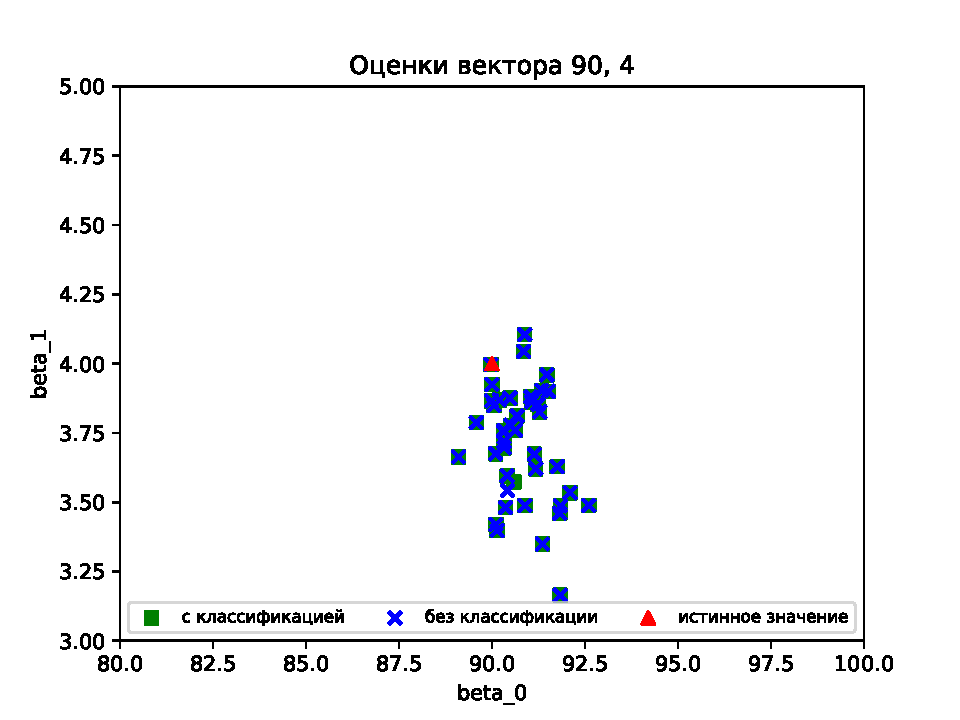
\includegraphics[width=110mm]{../images/plot_90_4_with-without_(3).pdf}
    \caption{График рассеяния $(\hat{\beta}_0,\hat{\beta}_1)$\label{overflow}}
    \label{pic4}
\end{figure}

Для построения рисунка \ref{pic5} генерировались выборки объема $N = 1000$. Доля выбросов $\widetilde{\varepsilon}$ равнялась $0.08$. 
Параметры регрессии выбирались $(90, 4)^T$. 
Регрессоры $x_i$ выбирались из равномерного распределения $\sim U(-5,5)$. 
Ошибки экспериментов подчинялись нормальному закону распределения с параметрами $(0, 16)$. Выбросы подчинялись нормальному распрелению с параметрами $(100, 100)$. 
\newpage

\begin{figure}[h]
    \centering
    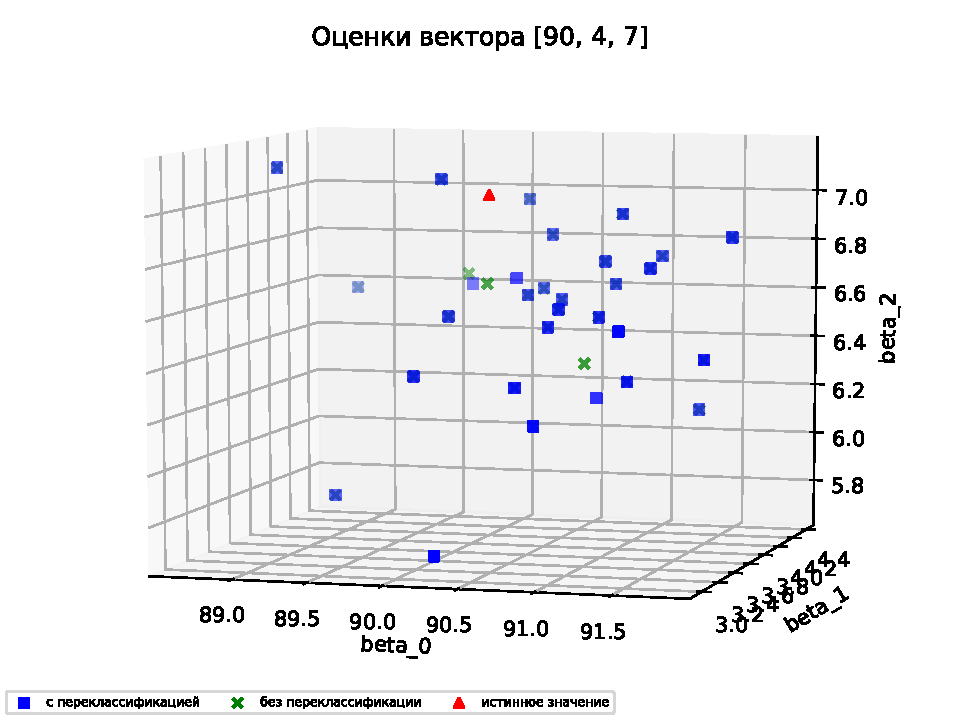
\includegraphics[width=100mm]{../images/plot_90_4_7_(4).pdf}
    \caption{График рассеяния $(\hat{\beta}_0,\hat{\beta}_1, \hat{\beta}_2)$\label{overflow}}
    \label{pic5}
\end{figure}

На полученных рисунках видно, что оценки параметров получаются близкими при разных выборках.

\subsection{Сравнение оценок при переклассификации методом K-ближайших соседей с оценками без переклассификации}
Были проведены эксперименты для сравнения эмпирической вариации оценок максимального правдоподобия, когда использовалась переклассификация методом K-ближайших соседей и когда не использовалась. При этом на каждой итерации выборка увеличивалась. 

Объем выборки $N$ изменялся от $N_1=100$ до $N_2=400$, при этом выборка дополнялась, а не генерировалась новая. Использовалась модель линейной регрессии. Доля выбросов была постоянна и равнялась $\widetilde{\varepsilon}=0.08$. Параметры регрессии были постоянными и равнялись $\beta=(90,4)^T$. 
Регрессоры $x_i$ были из равномерного распределения $U(-5,5)$, ошибки эспериментов $\varepsilon_i\sim \mathcal{N}(0,16)$. В методе, где использовалась переклассификация, величина $K$ выбиралась: $K=10$.
\newpage
\vspace{3cm}
\begin{center}
    \captionof{table}{Параметры модели и оценок экспериментов}\label{tab1}
    \begin{tabular}{|p{5cm}|p{5cm}|}
        \hline
        \multicolumn{2}{|c|}{Параметры программы} \\
        \hline
        Переменная&значение\\
        \hline
        Размер выборки $N$& от 100 до 400\\
        \hline
        Доля выбросов $\widetilde{\varepsilon}$& 0.08\\
        \hline
        Параметры регрессии $\beta$& $(90,4)$\\
        \hline
        Регрессоры $x_i$ & $\sim U(-5,5)$\\
        \hline
        $\varepsilon_i$&$\sim \mathcal{N}(0,16)$\\
        \hline
        $\eta_i$&$\sim \mathcal{N}(100,100)$\\
        \hline
        В методе, с переклассификацией величина $K$& 10\\
        \hline
    \end{tabular},
\end{center}

\begin{figure}[ht!]
    \centering
    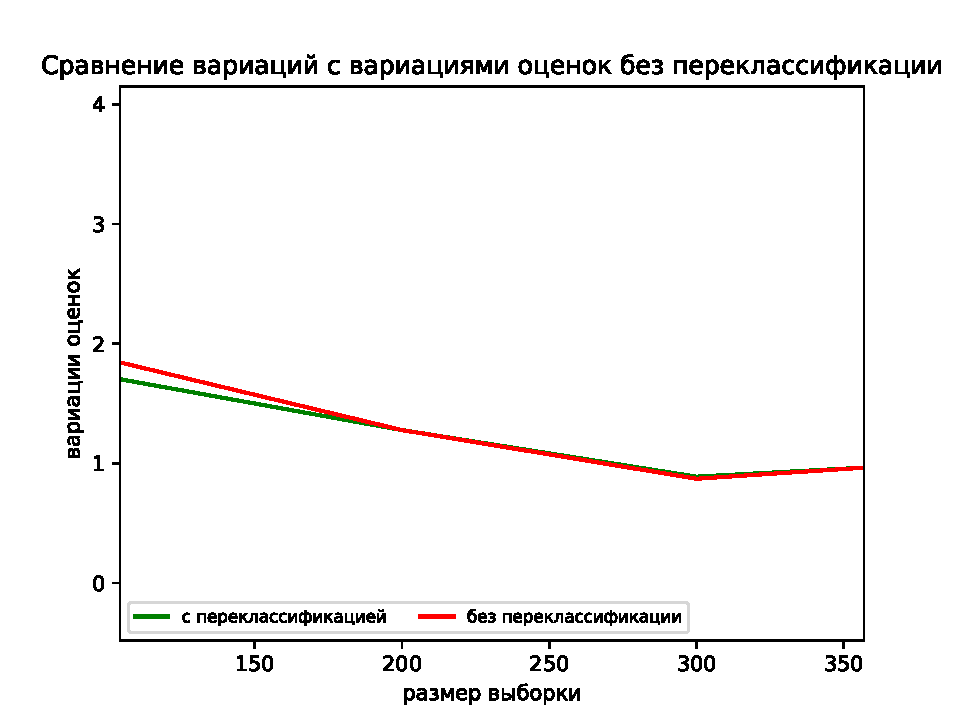
\includegraphics[width=100mm]{../images/on_off_recl.pdf}
    \caption{Сравнение вариаций оценок максимального правдоподобия когда используется и не используется переклассификация\label{overflow}}
    \label{pic2}
\end{figure}

% \subsection{Параметры модели и оценок}
% В ходе экспериментов использовались следующие параметры модели:
% \begin{center}
%     \begin{tabular}{|p{5cm}|p{5cm}|}
%         \hline
%         \multicolumn{2}{|c|}{Параметры программы} \\
%         \hline
%         Переменная&значение\\
%         \hline
%         Размер выборки $N$& 1000\\
%         \hline
%         Доля выбросов $\widetilde{\varepsilon}$& 0.08\\
%         \hline
%         Параметры регрессии $\beta$& $(90,4)$\\
%         \hline
%         Регрессоры $x_i$ & $\sim U(-5,5)$\\
%         \hline
%         $\varepsilon_i$&$\sim N(0,16)$\\
%         \hline
%         $\eta_i$&$\sim N(100,100)$\\
%         \hline
%         Величина $K$ из пункта 2.3 курсового проекта &$10$\\
%         \hline
%     \end{tabular},
% \end{center}
% \newpage

\subsection{Сравнительный анализ оценок максимального правдоподобия с альтернативной} \label{ss_4_6}
\subsubsection{Эксперимент с изменением объема выборки}
В следующем эксперименте был произведен сравнительный анализ вариаций ОМП-оценок с МНК оценками в зависимости от объема выборки.

Объем выборки $N$ изменялся от $N_1=100$ до $N_2=500$, при этом выборка дополнялась, а не генерировалась новая. Использовалась модель линейной регрессии. Доля выбросов была постоянна и равнялась $\widetilde{\varepsilon}=0.08$. Параметры регрессии были постоянными и равнялись $\beta=(90,4)^T$. 
Регрессоры $x_i$ были из равномерного распределения $U(-5,5)$, ошибки эспериментов $\varepsilon_i\sim \mathcal{N}(0,16)$. Для переклассификации использовался метод $K$-ближайших соседей.

\begin{center}
    \captionof{table}{Параметры модели и оценок}\label{tab1}
    \begin{tabular}{|p{5cm}|p{5cm}|}
        \hline
        \multicolumn{2}{|c|}{Параметры программы} \\
        \hline
        Переменная&значение\\
        \hline
        Размер выборки $N$& от 100 до 500\\
        \hline
        Доля выбросов $\widetilde{\varepsilon}$& 0.08\\
        \hline
        Параметры регрессии $\beta$& $(90,4)$\\
        \hline
        Регрессоры $x_i$ & $\sim U(-5,5)$\\
        \hline
        $\varepsilon_i$&$\sim \mathcal{N}(0,16)$\\
        \hline
        $\eta_i$&$\sim \mathcal{N}(100,100)$\\
        \hline
        Величина $K$  &$10$\\
        \hline
    \end{tabular},
\end{center}
\begin{figure}[h!]
    \centering
    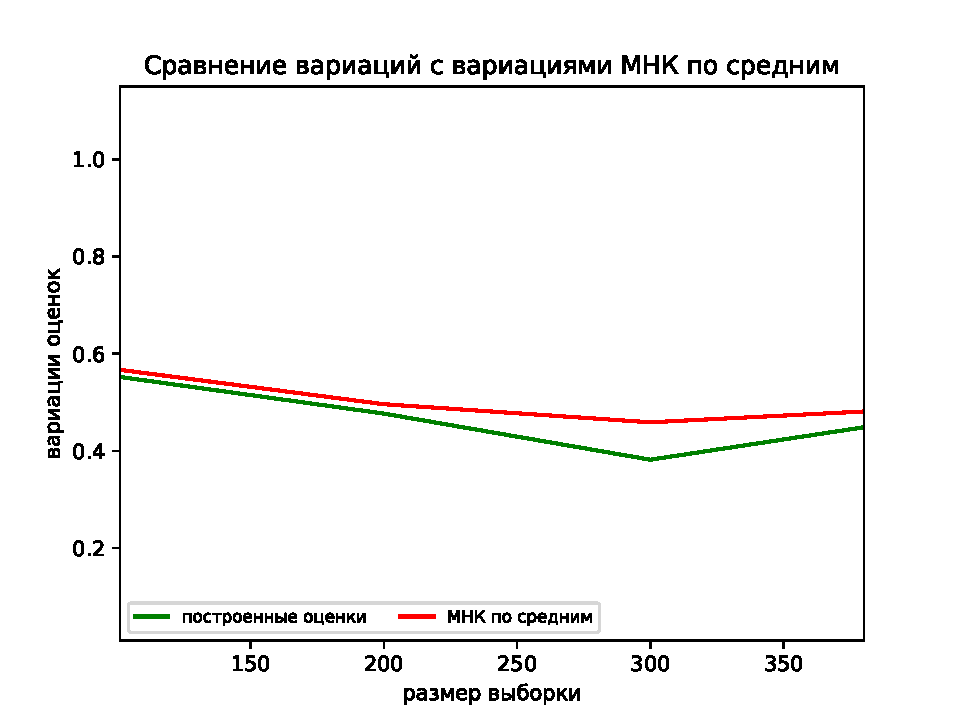
\includegraphics[width=100mm]{../images/OLS_GEM.pdf}
    \caption{Сравнение вариаций оценок\label{overflow}}
    \label{pic0}
\end{figure}
При сравнении графиков вариаций (рис.\ref{pic0}) можно сделать вывод, что ОМП дают лучший результат, 

\subsubsection{Эксперимент с полиномиальной регрессией}
Был проведен эксперимент с полиномиальной регрессией. Использовались те же параметры модели (таблица \ref{tab1}), объем выборки $N$ изменялся от 100 до 1000:
\newpage
\begin{figure}[h!]
    \centering
    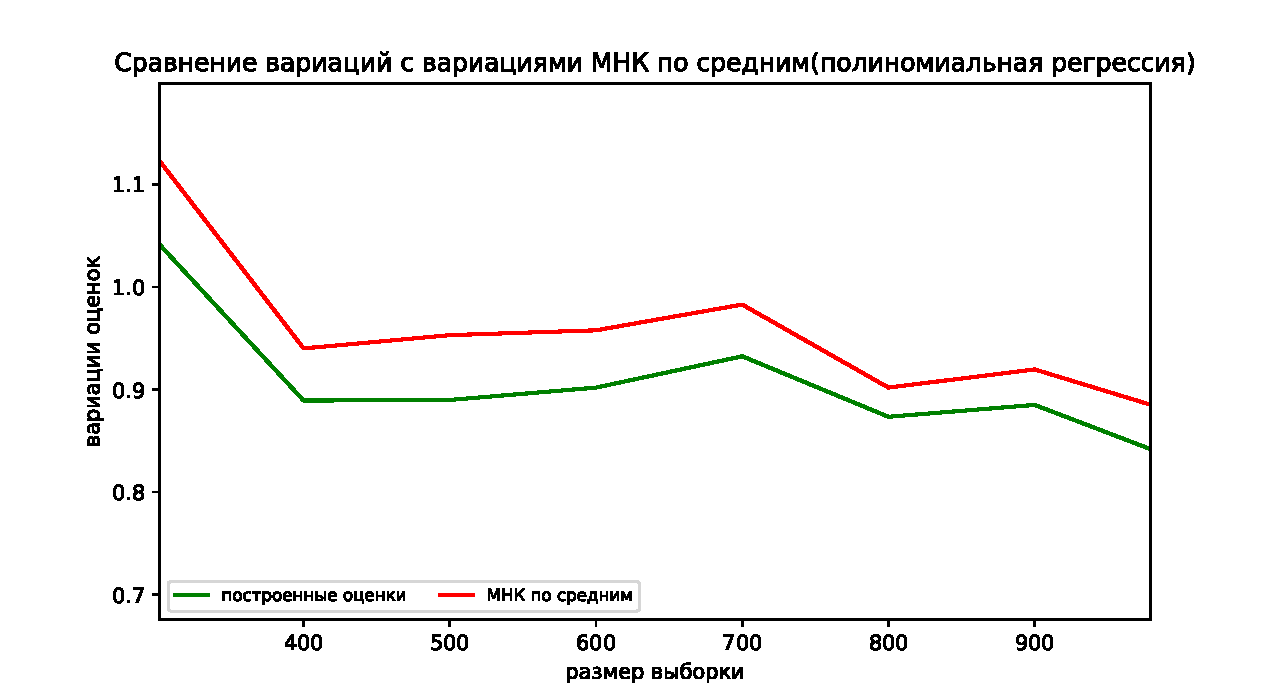
\includegraphics[width=150mm]{../images/polynomial.pdf}
    \caption{Вариации оценок в случае полиномиальной регрессии\label{overflow}}
    \label{pic3}
\end{figure}

Оба метода имели схожее поведение при изменении объема выборки, но построенные оценки максимального правдоподобия стабильно показывали лучший результат.

\subsection{Эксперименты с изменением уровня переклассификации выборки для метода $K$-ближайших соседей}\label{ss3_3_1}
В ходе дипломной работы были построены эксперименты с изменением величины K для метода $K$-ближайших соседей, используемого в переклассификации.  

Объем выборки $N$ был постоянным: $N=500$. Использовалась модель линейной регрессии. Доля выбросов была постоянна и равнялась $\widetilde{\varepsilon}=0.08$. Параметры регрессии были постоянными и равнялись $\beta=(90,4)^T$. 
Регрессоры $x_i$ были из равномерного распределения $U(-5,5)$, ошибки эспериментов $\varepsilon_i\sim \mathcal{N}(0,16)$. Величина $K$ менялась от $10$ до $40$.
\newpage
\begin{center}
    \captionof{table}{Параметры модели и оценок экспериментов с переклассификацией выборки}\label{tab1}
    \begin{tabular}{|p{5cm}|p{5cm}|}
        \hline
        \multicolumn{2}{|c|}{Параметры программы} \\
        \hline
        Переменная&значение\\
        \hline
        Размер выборки $N$& 500\\
        \hline
        Доля выбросов $\widetilde{\varepsilon}$& 0.08\\
        \hline
        Параметры регрессии $\beta$& $(90,4)$\\
        \hline
        Регрессоры $x_i$ & $\sim U(-5,5)$\\
        \hline
        $\varepsilon_i$&$\sim \mathcal{N}(0,16)$\\
        \hline
        $\eta_i$&$\sim \mathcal{N}(100,100)$\\
        \hline
        Величина $K$  &от $10$ до $40$\\
        \hline
    \end{tabular},
\end{center}

\begin{figure}[h!]
    \centering
    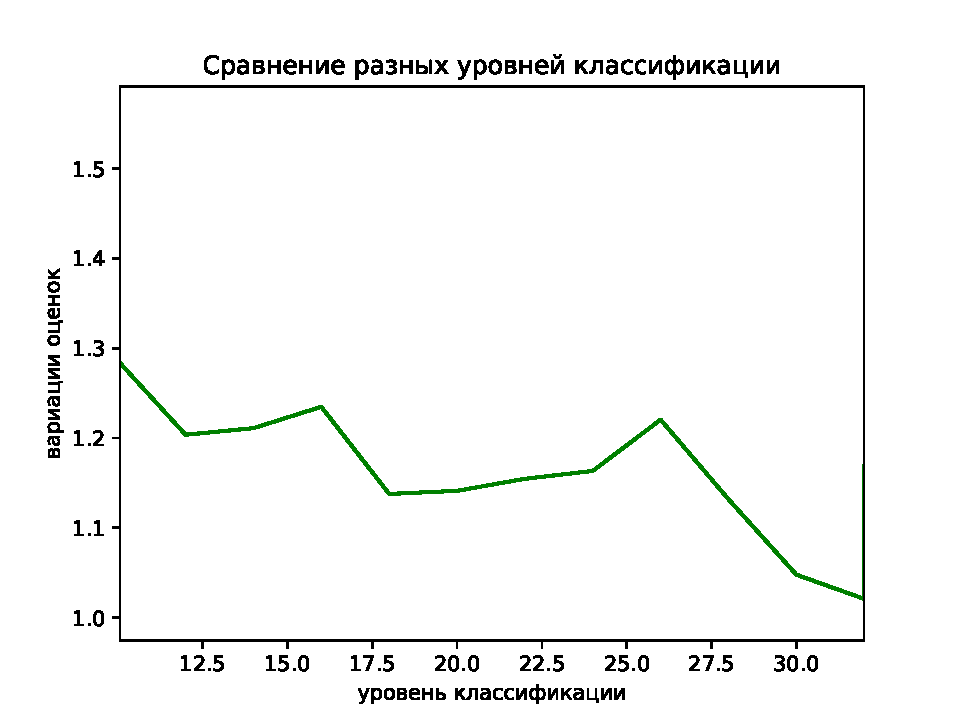
\includegraphics[width=100mm]{../images/different_recl_level.pdf}
    \caption{Зависимость вариаций от $K$ -- числа соседей, используемого в переклассификации выборки\label{overflow}}
    \label{pic1}
\end{figure}

В результате получилось, что при увеличении константы K точность оценки параметров растёт. 

\subsection{Эксперименты с изменением K для Local outlier factor, используемого в переклассификации}\label{ss3_3_2}
В ходе экспериментов была построена таблица, где выписаны $K$ для выборки определенного объема с определенной длиной интервала, то есть такую величину $K$, при которой количество неверных классов после переклассификации не более чем такое количество до переклассификации (значения получены опытным путём).
Доля выбросов была постоянна и равнялась $\widetilde{\varepsilon}=0.08$. Параметры регрессии были постоянными и равнялись $\beta=(90,4)^T$. 
Регрессоры $x_i$ были из равномерного распределения $U(-5,5)$, ошибки эспериментов $\varepsilon_i\sim \mathcal{N}(0,16)$.

\begin{center}
    \captionof{table}{Подходящие значения $K$ для выборки определенного объема с определенной длиной интервала}\label{tab2}
    \begin{tabular}{|p{5cm}|p{5cm}|p{5cm}|}
        \hline
        Объем выборки&длина интервала& величина $K$\\
        \hline
        1000 & 2.0 & 2\\
        1000 & 3.0 & 4\\
        1000 & 4.0 & 4\\

        3000 & 1.0 & 2\\
        3000 & 1.5 & 2\\
        3000 & 1.75 & 3\\
        3000 & 2.0 & 5\\
        3000 & 4.0 & 7\\

        10000 & 1.0 & 2\\
        10000 & 1.5 & 3\\
        10000 & 2.0 & 6\\
        10000 & 4.0 & 8\\
        \hline
    \end{tabular},
\end{center}
Далее приведен пример получаемых в ходе экспериментов значений.
было смоделировано $10^5$ наблюдений. Процент аномальных наблюдений: $8\%$. Константа $K$ равнялась 3.
\begin{Verbatim}[fontsize=\scriptsize]
    modulated with outlier count: 8047
    fit: classified
    wrong outliers: 7987
    fit: reclassificator scored 0.925034 on learning set:
    fit: reclassified 10
    
    fit: classified
    
    Classes differ with/without outliers when without reclassification: 7604
    Classes differ with/without outliers when with reclassification: 7582
\end{Verbatim}

Число 8047 - количество выбросов в выборке.

Число 7987 - количество ошибочно определенных выбросов (то есть ошибки рода: отнести выбросы к истинным значениям или истинные значения к выбросам). Хотим, чтобы было по крайней мере меньше предыдущего значения.

Число 7604 - количество неверных значений изначально, то есть неверных значений, полученных извне (это число может быть меньше 8047 так как при достаточно широких классах выбросы могли попасть в нужный класс)

Число 7582 - результат переклассификации, который мы хотим получить меньше предыдущего числа (7604). Чем меньше - тем лучше.


\subsection{Влияние переклассификации методом LOF на вариации оценок} \label{ss_4_9}
На следующем графике показано изменение вариаций ОМП и ОМП с переклассификацией методом, где используется локальный уровень выброса и случайный лес.
Объем выборки изменялся от $N=500$ до $N=800$. 
Доля выбросов $\widetilde{\varepsilon}$ равнялась $0.08$. 
Параметры регрессии выбирались $(90, 4)^T$. 
Регрессоры $x_i$ выбирались из равномерного распределения $\sim U(-5,5)$. 
Ошибки экспериментов подчинялись нормальному закону распределения с параметрами $(0, 16)$. Выбросы подчинялись нормальному распрелению с параметрами $(100, 100)$. 

\begin{figure}[hb]
    \centering
    \includegraphics[width=100mm]{../images/LOF_without(1).pdf}
    \caption{Зависимость вариаций от размера выборки\label{overflow}}
\end{figure}

На данном графике видно, что возможна сходимость оценок, а также в целом видно, что переклассификация очень хорошо влияет на точность результатов.

\newpage

\newpage

\newpage

\begin{center}
    \section*{Заключение}
\end{center}
\phantomsection
\addcontentsline{toc}{section}{Заключение}

По проведенным экспериментам видно, что оценки показывают не хуже результаты, чем альтернативные оценки, поэтому их можно рассматривать к использованию.
Можно добиться более точных результатов аппроксимации, если хорошо подобрать параметры оценок.
\newpage

\newpage
\addcontentsline{toc}{section}{Список Литературы}
\begin{thebibliography}{8}
    \bibitem{Huber}
    Хьюбер Дж П.~
    \textit{Робастность в статистике:пер. с англ.} --
    М.:Мир, 1984.-304 с.

    \bibitem{Kharin}
    Харин Ю.С., Зуев Н.М.,
    Жук Е.Е.~
    \textit{Теория вероятностей, математическая и прикладная статистика: учебник} --
    Минск: БГУ, 2011.-463 с.

    

    \bibitem{OLSforGrouping}
    Е. С Агеева, чл.-корр. НАН Беларуси Ю.С. Харин~
    \textit{Состоятельность оценки максимального правдопобия параметров множественной регрессии по классифицированным наблюдениям}

    \bibitem{RobustRegression}
    John Fox, Sanford Weisberg~
    \textit{Robust Regression} --
    October 8, 2013

    \bibitem{RobustPolynomialEstimation}
    А.В. Омельченко~
    \textit{Робастное оценивание параметров полиномиальной регрессии второго порядка} --
    Харьковский национальный университет радиоэлектроники, Украина, 2009

    \bibitem{ComparisonRobust}
    \"{O}zlem G\"{u}r\"{u}nl\"{u} Alma~
    \textit{Comparison of Robust Regression Methods
    in Linear Regression} -- 
    Int. J. Contemp. Math. Sciences, Vol. 6, 2011, no. 9, 409 - 421 с.

    \bibitem{Winitzki}
    Sergei Winitzki~
    \textit{A handy approximation for the error function and its inverse.}

    \bibitem{NumericalMethods}
    Мандрик П.А., Репников В.И., Фалейчик Б.В.,
    \textit{Численные методы} [Электронный ресурс].

    \bibitem{interval_valued}
    Paolo Giordani~
    \textit{Linear regression analysis for interval-valued data based on the Lasso technique} --
    Department of Statistical Sciences Sapienza University of Rome

    \bibitem{minkowski}
    Masahiro Inuiguchi, Tetsuzo Tanino,~
    \textit{interval linear regression methods based on minkowski difference a bridge between traditional and interval linear regression models.} --
    KYBERNETIKA, volume 42, 2006 , number 4, pages 423 - 440

    \bibitem{technometrics}
     Nelson, W., Hahn, G.J.~
    \textit{Technometrics}. 
    volume 14, 1972, pages 247–269.
\end{thebibliography}
\newpage

\section*{Приложение}
\phantomsection
\addcontentsline{toc}{section}{Приложение}

Метод наименьших квадратов по центрам интервалов
\begin{Verbatim}[fontsize=\scriptsize]
    class ApproximationGEMModelNaive(ApproximationGEMModelRedesigned):
        def fit(self):
            self.classify()
    
            def ex_generator(mu_data):
                for i in range(0, self.endogen.size):
                    if mu_data[i] is None:
                        continue
                    a_mu_i_plus_1 = mu_data[i] * Defines.INTERVAL_LENGTH
                    a_mu_i = mu_data[i] * Defines.INTERVAL_LENGTH - Defines.INTERVAL_LENGTH
                    yield (a_mu_i_plus_1 + a_mu_i) / 2
    
            naive_ex_data_positive = np.fromiter(ex_generator(self._np_freq_positive), float)
            naive_ex_data_negative = np.fromiter(ex_generator(self._np_freq_negative), float)
    
            naive_ex_data_full = np.append(naive_ex_data_positive, naive_ex_data_negative)
    
            z, resid, rank, sigma = np.linalg.lstsq(self.exogen, naive_ex_data_full, rcond=None)
            return z
\end{Verbatim}

Моделирование полиномиальной регрессии:
\begin{Verbatim}[fontsize=\scriptsize]
def modulate_polynomial_regression(regression_sample_quintity, regression_outlier_percentage):
    regression_parameters = ACCURATE_RESULT
    _x_points = np.zeros(shape=[regression_sample_quintity, len(regression_parameters)])
    _y_points = np.zeros(shape=regression_sample_quintity)

    def np_random_polynomial(size):
        _res = np.zeros(size)
        for i in range(0, size):
            _res[i] = random.uniform(-5, 5) ** (i + 1)

        return _res

    for i in range(0, regression_sample_quintity):
        _x_points[i] = np.append(np.ones(1), np_random_polynomial(len(ACCURATE_RESULT) - 1))
        if random.random() > regression_outlier_percentage / 100:
            _y_points[i] = (_x_points[i] * ACCURATE_RESULT) + np.random.normal(0, 4)
        else:
            _y_points[i] = np.random.normal(100.0, 15.0, size=1)

    return _x_points, _y_points
\end{Verbatim}

Моделирование линейной регрессии:
\begin{Verbatim}[fontsize=\scriptsize]
    def modulateRegression(regression_sample_quintity, regression_outlier_percentage):
    regression_parameters = ACCURATE_RESULT
    _x_points = np.zeros(shape=[regression_sample_quintity, len(regression_parameters)])
    _y_points = np.zeros(shape=regression_sample_quintity)

    for i in range(0, regression_sample_quintity):
        if random.random() > regression_outlier_percentage / 100:
            _x_points[i] = np.append(np.ones(1), np.random.uniform(-5, 5, size=len(regression_parameters) - 1))
            _y_points[i] = (_x_points[i] * regression_parameters) + np.random.normal(0, 4)
        else:
            _x_points[i] = np.append(np.ones(1), np.random.uniform(-5, 5, size=len(regression_parameters) - 1))
            _y_points[i] = np.random.normal(100.0, 15.0, size=1)

    return _x_points, _y_points
\end{Verbatim}

\textit{Метод наименьших квадратов по центрам интервалов}:
\begin{Verbatim}[fontsize=\scriptsize]

def fit_data_naive_classic():
    sample_sizes = []
    all_results_classic = []
    all_results_naive = []
    for sample_size in range(SAMPLE_SIZE_MIN, SAMPLE_SIZE_MAX+1, SAMPLE_SIZE_STEP):
        successful_fit = False
        while not successful_fit:
            x_points, y_points = modulateRegression(sample_size, OUTLIER_PERCENTAGE)
            approx_model = groupingEstimates.GEM(x_points, y_points)
            approx_model_naive = groupingEstimatesNaive.GEM_N(x_points, y_points)
            try:
                result = approx_model.fit()
                print("GEM {}".format(result))
                result_naive = approx_model_naive.fit()
                print("GEM_N {}".format(result_naive))

                successful_fit = True

                all_results_classic.append(result)
                all_results_naive.append(result_naive)
                sample_sizes.append(sample_size)
            except KeyboardInterrupt:
                print("stopping...")
                np.save(NP_DATA_PATH + "gem_res_classic", all_results_classic)
                np.save(NP_DATA_PATH + "gem_res_naive", all_results_naive)
                np.save(NP_DATA_PATH + "gem_sizes", sample_sizes)
                quit()
            except Exception as e:
                print(e)
    np.save(NP_DATA_PATH + "gem_res_classic", all_results_classic)
    np.save(NP_DATA_PATH + "gem_res_naive", all_results_naive)
    np.save(NP_DATA_PATH + "gem_sizes", sample_sizes)

\end{Verbatim}

График с разным объемом выборки:
\begin{Verbatim}[fontsize=\scriptsize]
def plot_with_different_sample_size():
    sample_sizes = []
    all_results_with_classification = []
    all_results_without_classification = []

    x_points = None
    y_points = None

    for sample_size in range(SAMPLE_SIZE_MIN, SAMPLE_SIZE_MAX+1, SAMPLE_SIZE_STEP):
        successful_fit = False
        while not successful_fit:
            x_points_t, y_points_t = modulateRegression(sample_size, OUTLIER_PERCENTAGE)

            if x_points is None or y_points is None:
                x_points = x_points_t
                y_points = y_points_t
            else:
                x_points = np.append(x_points, x_points_t, axis=0)
                y_points = np.append(y_points, y_points_t, axis=0)

            approx_model = groupingEstimates.GEM(x_points, y_points)
            try:
                result = approx_model.fit()
                print("GEM {}".format(result))
                result_without = approx_model.fit_without_reclassification()
                print("GEM_without {}".format(result_without))

                successful_fit = True

                all_results_with_classification.append(result)
                all_results_without_classification.append(result_without)
                sample_sizes.append(sample_size)
            except KeyboardInterrupt:
                print("stopping...")
                np.save(NP_DATA_PATH + "gem_res_with", all_results_with_classification)
                np.save(NP_DATA_PATH + "gem_res_without", all_results_without_classification)
                np.save(NP_DATA_PATH + "gem_sizes_with_without", sample_sizes)
                quit()
            except Exception as e:
                print(e)
    np.save(NP_DATA_PATH + "gem_res_with", all_results_with_classification)
    np.save(NP_DATA_PATH + "gem_res_without", all_results_without_classification)
    np.save(NP_DATA_PATH + "gem_sizes_with_without", sample_sizes)

\end{Verbatim}

График с разным уровнем переклассификации:
\begin{Verbatim}[fontsize=\scriptsize]
def plot_with_different_reclassification_level():
    reclassification_levels = []
    all_results_with_classification = []
    recl_level_min = 10
    recl_level_max = 40

    x_points, y_points = modulateRegression(500, OUTLIER_PERCENTAGE)

    for recl_level in range(recl_level_min, recl_level_max + 1, 2):
        GroupingEstimatesDefines.RECLASSIFICATION_LEVEL = recl_level

        successful_fit = False
        while not successful_fit:
            approx_model = groupingEstimates.GEM(x_points, y_points)
            try:
                result = approx_model.fit()
                print("GEM {}".format(result))

                successful_fit = True

                all_results_with_classification.append(result)
                reclassification_levels.append(recl_level)
            except KeyboardInterrupt:
                print("stopping...")
                np.save(NP_DATA_PATH + "gem_with_dif_level_results", all_results_with_classification)
                np.save(NP_DATA_PATH + "gem_with_dif_level_levels", reclassification_levels)
                quit()
            except Exception as e:
                print(e)
    np.save(NP_DATA_PATH + "gem_with_dif_level_results", all_results_with_classification)
    np.save(NP_DATA_PATH + "gem_with_dif_level_levels", reclassification_levels)

\end{Verbatim}

\end{document}